\chapter{Stochastic Processes in Continuous Time}
\label{chap:stochastic-processes-continuous-time}

\section{General Notions}
\label{sec:general-notions}

The following definitions are straightforward extensions of those introduced earlier for sequences of random variables, the underlying idea being that of a family of random variables depending on time.

\begin{Definition}[Stochastic Process]
\label{def:stochastic-process}
A stochastic process is a family of random variables $\xi(t)$ parametrized by $t \in T$, where $T \subset \mathbb{R}$. When $T = \{1, 2, \ldots\}$, we shall say that $\xi(t)$ is a stochastic process in discrete time (i.e. a sequence of random variables). When $T$ is an interval in $\mathbb{R}$ (typically $T = [0, \infty)$), we shall say that $\xi(t)$ is a stochastic process in continuous time.
\end{Definition}

For every $\omega \in \Omega$ the function
\[
T \ni t \mapsto \xi(t, \omega)
\]
is called a path (or sample path) of $\xi(t)$.

\begin{Definition}[Filtration]
\label{def:filtration}
A family $\mathcal{F}_t$ of $\sigma$-fields on $\Omega$ parametrized by $t \in T$, where $T \subset \mathbb{R}$, is called a filtration if
\[
\mathcal{F}_s \subset \mathcal{F}_t \subset \mathcal{F}
\]
for any $s, t \in T$ such that $s \leq t$.
\end{Definition}

\begin{Definition}[Martingale]
\label{def:martingale}
A stochastic process $\xi(t)$ parametrized by $t \in T$ is called a martingale (submartingale, supermartingale) with respect to a filtration $\mathcal{F}_t$ if
\begin{enumerate}
\item $\xi(t)$ is integrable for each $t \in T$;
\item $\xi(t)$ is $\mathcal{F}_t$-measurable for each $t \in T$ (in which case we say that $\xi(t)$ is adapted to $\mathcal{F}_t$);
\item $\xi(s) = E(\xi(t) \mid \mathcal{F}_s)$ (respectively, $\leq$ or $\geq$) for every $s, t \in T$ such that $s \leq t$.
\end{enumerate}
\end{Definition}

In earlier chapters we have seen various stochastic processes, in particular, martingales in discrete time such as the symmetric random walk, for example. In what follows we shall study in some detail two processes in continuous time, namely, the Poisson process and Brownian motion.

\section{Poisson Process}
\label{sec:poisson-process}

\subsection{Exponential Distribution and Lack of Memory}
\label{sec:exponential-distribution}

\begin{Definition}[Exponential Distribution]
\label{def:exponential-distribution}
We say that a random variable $\eta$ has the exponential distribution of rate $\lambda > 0$ if
\begin{align}
P\{\eta > t\} = e^{-\lambda t}
\label{eq:exponential-tail}
\end{align}
for all $t \geq 0$.
\end{Definition}

For example, the emissions of particles by a sample of radioactive material (or calls made at a telephone exchange) occur at random times. The probability that no particle is emitted (no call is made) up to time $t$ is known to decay exponentially as $t$ increases. That is to say, the time $\eta$ of the first emission has the exponential distribution, $P\{\eta > t\} = e^{-\lambda t}$.

\begin{Exercise}
\label{ex:exponential-distribution-function}
What is the distribution function of a random variable $\eta$ with exponential distribution? Does it have a density? If so, find the density.

\noindent\textbf{Hint:} What is the probability that $\eta > 0$? What is the probability that $\eta > t$ for any given $t < 0$? Can you express the distribution function in terms of $P\{\eta > t\}$? Is the distribution function differentiable?
\end{Exercise}

\begin{Exercise}
\label{ex:exponential-expectation-variance}
Compute the expectation and variance of a random variable having the exponential distribution.

\noindent\textbf{Hint:} Use the density found in Exercise~\ref{ex:exponential-distribution-function}.
\end{Exercise}

\begin{Exercise}
\label{ex:exponential-functional-equation}
Show that a random variable $\eta$ with exponential distribution satisfies
\begin{equation}
P\{\eta > t + s\} = P\{\eta > t\} P\{\eta > s\} \tag{6.1}
\end{align}
for any $s, t \geq 0$.

\noindent\textbf{Hint:} When the probabilities are replaced by exponents, the equality should become obvious.
\end{Exercise}

\begin{Exercise}
\label{ex:lack-of-memory-equivalent}
Show that the equality in Exercise~\ref{ex:exponential-functional-equation} is equivalent to
\begin{align}
P\{\eta > t + s \mid \eta > s\} = P\{\eta > t\} \tag{6.2}
\end{align}
for any $s, t \geq 0$.

\noindent\textbf{Hint:} Recall how to compute conditional probability. Observe that $\eta > s + t$ implies $\eta > s$.
\end{Exercise}

The equality \cref{eq:lack-of-memory} (or, equivalently, \cref{eq:exponential-functional-equation}) is known as the \textbf{lack of memory property}. The odds that no particle will be emitted (no call will be made) in the next time interval of length $t$ are not affected by the length of time $s$ it has already taken to wait, given that no emission (no call) has occurred yet.

\begin{Exercise}
\label{ex:exponential-unique-lack-of-memory}
Show that the exponential distribution is the only probability distribution satisfying the lack of memory property.

\noindent\textbf{Hint:} The lack of memory property means that $g(t) = P\{\eta > t\}$ satisfies the functional equation
\[
g(t + s) = g(t) g(s)
\]
for any $s, t > 0$. Find all non-negative non-increasing solutions of this functional equation.
\end{Exercise}

\subsection{Construction of the Poisson Process}
\label{sec:poisson-process-construction}

Let $\eta_1, \eta_2, \ldots$ be a sequence of independent random variables, each having the same exponential distribution of rate $\lambda$. For example, the times between the emissions of radioactive particles (or between calls made at a telephone exchange) have this property. We put
\[
\xi_n = \eta_1 + \dots + \eta_n,
\]
which can be thought of as the time of the $n$-th emission (the $n$-th call). We also put $\xi_0 = 0$ for convenience. The number of emissions (calls) up to time $t \geq 0$ is an $n$ such that $\xi_{n+1} > t \geq \xi_n$. In other words, the number of emissions (calls) up to time $t \geq 0$ is equal to $\max\{n: t \geq \xi_n\}$.

\begin{Definition}[Poisson Process]
\label{def:poisson-process}
We say that $N(t)$, where $t \geq 0$, is a Poisson process if
\begin{align}
N(t) = \max\{n: t \geq \xi_n\}.
\label{eq:poisson-process-definition}
\end{align}
\end{Definition}

Thus, $N(t)$ can be regarded as the number of particles emitted (calls made) up to time $t$. It is an example of a stochastic process in continuous time. A typical path of $N(t)$ is shown in \cref{fig:poisson-path}. It begins at the origin, $N(0) = 0$ (no particles emitted at time 0), and is right-continuous, non-decreasing and piecewise constant with jumps of size 1 at the times $\xi_n$.

\begin{figure}[htbp]
\centering
\caption{A typical path of $N(t)$ and the jump times $\xi_n$}
\label{fig:poisson-path}
% 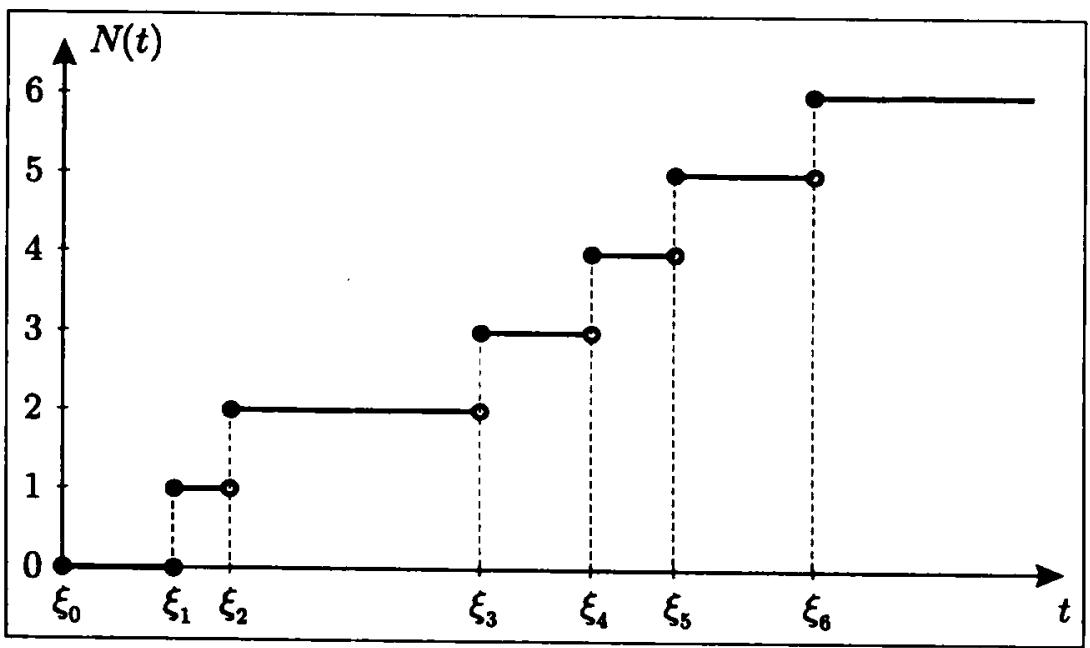
\includegraphics[]{images/chunk1_1f40ca443da34a651d89a8801aaf8963464978dbcbe17837d7207fdd68effde0.jpg}
\end{figure}

What is the distribution of $N(t)$? To answer this question we need to recall the definition of the Poisson distribution.

\begin{Definition}[Poisson Distribution]
\label{def:poisson-distribution}
A random variable $\nu$ has the Poisson distribution with parameter $\alpha > 0$ if
\begin{equation}
P\{\nu = n\} = e^{-\alpha} \frac{\alpha^n}{n!}
\label{eq:poisson-pmf}
\end{equation}
for any $n = 0, 1, 2, \ldots$
\end{Definition}

The probabilities $P\{\nu = n\}$ for various values of $\alpha$ are shown in \cref{fig:poisson-distribution}.

\begin{figure}[htbp]
\centering
\caption{Poisson distribution with parameter $\alpha$}
\label{fig:poisson-distribution}
% 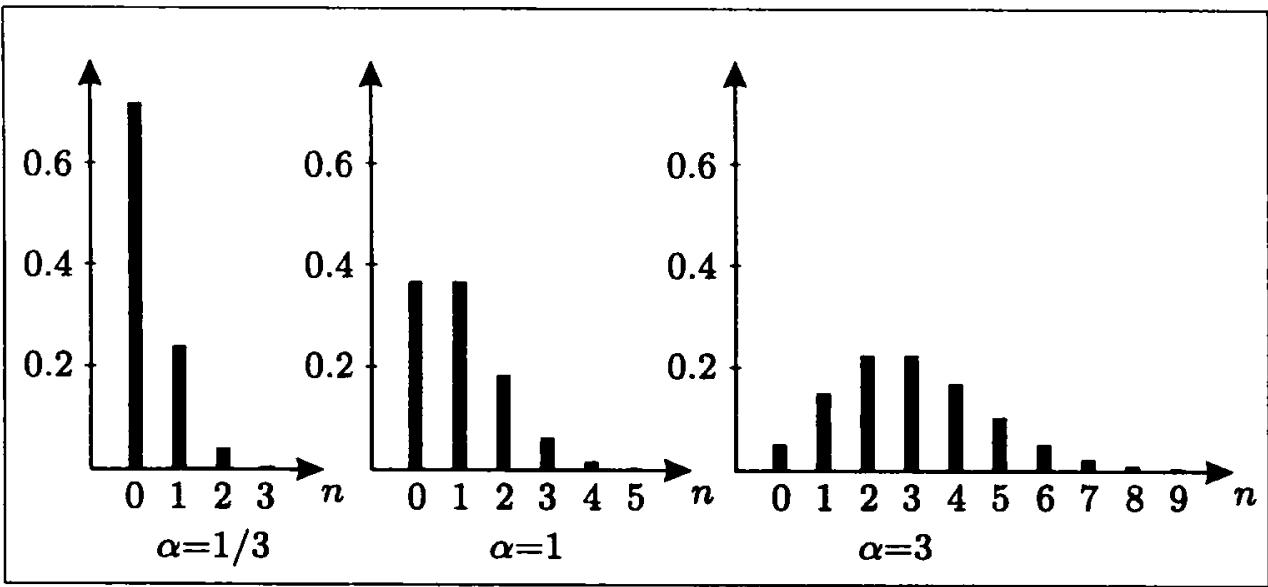
\includegraphics[]{images/chunk1_bc39f5ae4e6489ea1a68128efc52c079ab83ad777a589dedc1b315918e4e024c.jpg}
\end{figure}

\begin{Proposition}[Poisson Process Distribution]
\label{prop:poisson-process-distribution}
$N(t)$ has the Poisson distribution with parameter $\lambda t$,
\begin{equation}
P\{N(t) = n\} = e^{-\lambda t} \frac{(\lambda t)^n}{n!}.
\label{eq:poisson-process-pmf}
\end{equation}
\end{Proposition}

\begin{proof}
First of all, observe that
\begin{equation}
\{N(t) < n\} = \{\xi_n > t\}.
\label{eq:poisson-event-equivalence}
\end{equation}

It suffices to compute the probability of this event for any $n$ because
\begin{equation}
\begin{aligned}
P\{N(t) = n\} &= P\{N(t) < n + 1\} - P\{N(t) < n\} \\
&= P\{\xi_{n+1} > t\} - P\{\xi_n > t\}. \tag{6.3}
\end{align}

We shall prove by induction on $n$ that
\begin{align}
P\{\xi_n > t\} = e^{-\lambda t} \sum_{k=0}^{n-1} \frac{(\lambda t)^k}{k!}. \tag{6.4}
\end{align}

For $n = 1$:
\[
P\{\xi_1 > t\} = P\{\eta_1 > t\} = e^{-\lambda t}.
\]

Next, suppose that \cref{eq:xi-n-tail-probability} holds for some $n$. Then, expressing $\xi_{n+1}$ as the sum of the independent random variables $\xi_n$ and $\eta_{n+1}$, we compute
\begin{align}
\begin{aligned}
P\{\xi_{n+1} > t\} &= P\{\xi_n + \eta_{n+1} > t\} \\
&= P\{\eta_{n+1} > t\} + P\{\xi_n > t - \eta_{n+1}, t \geq \eta_{n+1} > 0\} \\
&= e^{-\lambda t} + \int_0^t P\{\xi_n > t - s\} f_{\eta_{n+1}}(s) \, ds \\
&= e^{-\lambda t} + \int_0^t e^{-\lambda(t-s)} \sum_{k=0}^{n-1} \frac{(\lambda(t-s))^k}{k!} \lambda e^{-\lambda s} \, ds \\
&= e^{-\lambda t} + e^{-\lambda t} \sum_{k=0}^{n-1} \frac{\lambda^{k+1}}{k!} \int_0^t (t-s)^k \, ds \\
&= e^{-\lambda t} \sum_{k=0}^n \frac{(\lambda t)^k}{k!},
\end{aligned}
\end{equation}
where $f_{\eta_{n+1}}(s)$ is the density of $\eta_{n+1}$. By induction, \cref{eq:xi-n-tail-probability} holds for any $n$. Now apply \cref{eq:poisson-probability-difference} to complete the proof.
\endproof
\end{Proposition}

\begin{Exercise}
\label{ex:poisson-expectation}
What is the expectation of $N(t)$?

\noindent\textbf{Hint:} What are the possible values of $N(t)$? What are the corresponding probabilities? Can you compute the expectation from these? To simplify the result use the Taylor expansion of $e^x$.
\end{Exercise}

\begin{Exercise}
\label{ex:poisson-joint-probability}
Compute $P\{N(s) = 1, N(t) = 2\}$ for any $0 \leq s < t$.

\noindent\textbf{Hint:} Express $\{N(s) = 1, N(t) = 2\}$ as $\{\eta_1 \leq s < \eta_1 + \eta_2 \leq t < \eta_1 + \eta_2 + \eta_3\}$. You can compute the probability of the latter, since $\eta_1, \eta_2, \eta_3$ are exponentially distributed and independent.
\end{Exercise}

\subsection{Poisson Process Starts from Scratch at Time $t$}
\label{sec:poisson-starts-from-scratch}

Imagine that you are to take part in an experiment to count the emissions of a radioactive particle. Unfortunately, in the excitement of proving the lack of memory property you forget about the engagement and arrive late to find that the experiment has already been running for time $t$ and you have missed the first $N(t)$ emissions. Determined to make the best of it, you start counting right away, so at time $t + s$ you will have registered $N(t + s) - N(t)$ emissions. It will now be necessary to discuss $N(t + s) - N(t)$ instead of $N(s)$ in your report.

What are the properties of $N(t+s) - N(t)$? Perhaps you can guess something from the physical picture? After all, a sample of radioactive material will keep emitting particles no matter whether anyone cares to count them or not. So the moment when someone starts counting does not seem important. You can expect $N(t+s) - N(t)$ to behave in a similar way as $N(s)$. And because radioactive emissions have no memory of the past, $N(t+s) - N(t)$ should be independent of $N(t)$.

To study this conjecture recall the construction of a Poisson process $N(t)$ based on a sequence of independent random variables $\eta_1, \eta_2, \ldots$, all having the same exponential distribution. We shall try to represent $N(t + s) - N(t)$ in a similar way.

Let us put
\begin{equation}
\eta_1^t := \xi_{N(t)+1} - t, \quad \eta_n^t := \eta_{N(t)+n}, \quad n = 2, 3, \ldots,
\label{eq:eta-t-definition}
\end{equation}
see \cref{fig:eta-t-definition}. These are the times between the jumps of $N(t+s) - N(t)$. Then we define
\begin{equation}
\xi_n^t = \eta_1^t + \dots + \eta_n^t,
\label{eq:xi-t-definition}
\end{equation}
\begin{equation}
N^t(s) = \max\{n: \xi_n^t \leq s\}.
\label{eq:n-t-definition}
\end{equation}

\begin{figure}[htbp]
\centering
\caption{The random variables $\eta_1^t, \eta_2^t, \eta_3^t, \ldots$}
\label{fig:eta-t-definition}
% 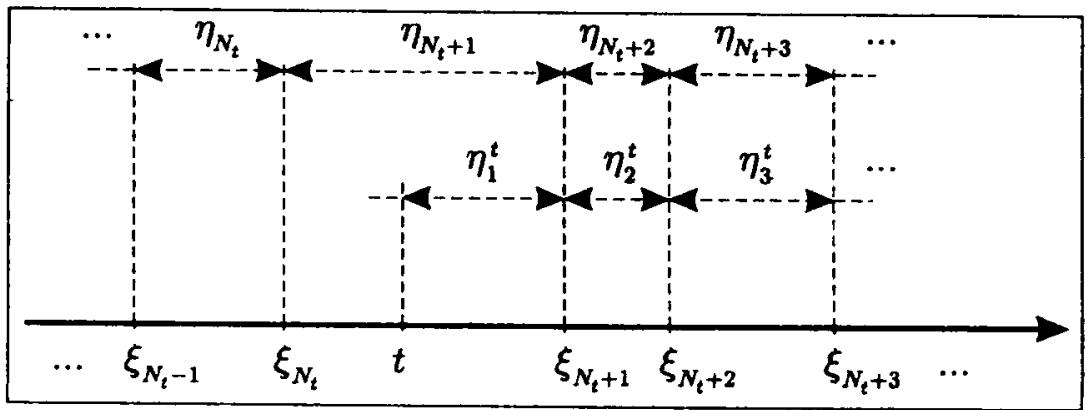
\includegraphics[]{images/chunk1_be6aef3a7dbce462fa2c720157d7ce29ddd76cbd3235850d9f62a801343d578b.jpg}
\end{figure}

\begin{Exercise}
\label{ex:n-t-equals-difference}
Show that
\begin{equation}
N^t(s) = N(t + s) - N(t).
\label{eq:n-t-equals-difference}
\end{equation}

\noindent\textbf{Hint:} First show that $\xi_n^t = \xi_{N(t)+n} - t$.
\end{Exercise}

If we can show that $\eta_1^t, \eta_2^t, \ldots$ are independent random variables having the same exponential distribution as $\eta_1, \eta_2, \ldots$, it will mean that $N(t + s) - N(t)$ is a Poisson process with the same probability distribution as $N(s)$. Moreover, if the $\eta_n^t$ turn out to be independent of $N(t)$, it will imply that $N(t + s) - N(t)$ is also independent of $N(t)$.

Before setting about this task beware of one common mistake. It is sometimes claimed that the times $\eta_1^t, \eta_2^t, \eta_3^t, \ldots$ between the jumps of $N(t + s) - N(t)$ are equal to $\xi_{n+1} - t, \eta_{n+2}, \eta_{n+3}, \ldots$ for some $n$. Hence $\eta_1^t, \eta_2^t, \eta_3^t, \ldots$ are independent because the random variables $\xi_{n+1}, \eta_{n+2}, \eta_{n+3}, \ldots$ are. The flaw in this is that, in fact, $\eta_1^t, \eta_2^t, \eta_3^t, \ldots$ are equal to $\xi_{n+1} - t, \eta_{n+2}, \eta_{n+3}, \ldots$ only on the set $\{N(t) = n\}$. However, the argument can be saved by conditioning with respect to $N(t)$. Our task becomes an exercise in computing conditional probabilities.

\begin{Exercise}
\label{ex:eta-t-tail-conditional}
Show that
\begin{equation}
P\{\eta_1^t > s \mid N(t)\} = P\{\eta_1 > s\}.
\label{eq:eta-t-tail-conditional}
\end{equation}

\noindent\textbf{Hint:} It suffices (why?) to verify that
\[
P\{\eta_1^t > s, N(t) = n\} = P\{\eta_1 > s\} P\{N(t) = n\}
\]
for any $n$. To this end, write the sets $\{N(t) = n\}$ and $\{\eta_1^t > s, N(t) = n\}$ in terms of $\xi_n$ and $\eta_{n+1}$, which are independent random variables, and use the lack of memory property for $\eta_{n+1}$.
\end{Exercise}

\begin{Exercise}
\label{ex:eta-t-independence}
Show that
\begin{equation}
P\{\eta_1^t > s_1, \ldots, \eta_k^t > s_k \mid N(t)\} = P\{\eta_1 > s_1\} \cdots P\{\eta_k > s_k\}.
\label{eq:eta-t-multivariate-conditional}
\end{equation}

\noindent\textbf{Hint:} Verify that
\[
P\{\eta_1^t > s_1, \eta_2^t > s_2, \ldots, \eta_k^t > s_k, N(t) = n\} = P\{\eta_1 > s_1\} \cdots P\{\eta_k > s_k\} P\{N(t) = n\}
\]
for any $n$. This is done in Exercise~\ref{ex:eta-t-tail-conditional} for $k = 1$.
\end{Exercise}

\begin{Exercise}
\label{ex:eta-t-distribution}
From the formula in Exercise~\ref{ex:eta-t-independence} deduce that the random variables $\eta_n^t$ and $N(t)$ are independent, and the $\eta_n^t$ have the same probability distribution as $\eta_n$, i.e. exponential with parameter $\lambda$.

\noindent\textbf{Hint:} What do you get if you take the expectation on both sides of the equality in Exercise~\ref{ex:eta-t-independence}? Can you deduce the probability distribution of $\eta_n^t$? Can you see that the $\eta_n^t$ are independent?

To prove that the $\eta_n^t$ are independent of $N(t)$ you need to be a little more careful and integrate over $\{N(t) = n\}$ instead of taking the expectation.
\end{Exercise}

Because $N(t + s) - N(t)$ can be defined in terms of $\eta_1^t, \eta_2^t, \ldots$ in the same way the original Poisson process $N(t)$ is defined in terms of $\eta_1, \eta_2, \ldots$, the result in Exercise~\ref{ex:eta-t-distribution} proves the theorem below.

\begin{Theorem}[Poisson Process Stationarity]
\label{thm:poisson-stationarity}
For any fixed $t \geq 0$
\[
N^t(s) = N(t + s) - N(t), \quad s \geq 0
\]
is a Poisson process independent of $N(t)$ with the same probability law as $N(s)$.
\end{Theorem}

That is to say, for any $s, t \geq 0$ the increment $N(t + s) - N(t)$ is independent of $N(t)$ and has the same probability distribution as $N(s)$. The assertion can be generalized to several increments, resulting in the following important theorem.

\begin{Theorem}[Poisson Process Independent Increments]
\label{thm:poisson-independent-increments}
For any $0 \leq t_1 \leq t_2 \leq \cdots \leq t_n$ the increments
\[
N(t_1), N(t_2) - N(t_1), N(t_3) - N(t_2), \ldots, N(t_n) - N(t_{n-1})
\]
are independent and have the same probability distribution as
\[
N(t_1), N(t_2 - t_1), N(t_3 - t_2), \ldots, N(t_n - t_{n-1}).
\]
\end{Theorem}

\beginproof
From \cref{thm:poisson-stationarity} it follows immediately that each increment $N(t_i) - N(t_{i-1})$ has the same distribution as $N(t_i - t_{i-1})$ for $i = 1, \ldots, n$.

It remains to prove independence. This can be done by induction. The case when $n = 2$ is covered by \cref{thm:poisson-stationarity}. Now suppose that independence holds for $n$ increments of a Poisson process for some $n \geq 2$. Take any sequence
\[
0 \leq t_1 \leq t_2 \leq \dots \leq t_n \leq t_{n+1}.
\]

By the induction hypothesis
\[
N(t_{n+1}) - N(t_n), \ldots, N(t_2) - N(t_1)
\]
are independent, since they can be regarded as increments of
\[
N^{t_1}(s) = N(t_1 + s) - N(t_1),
\]
which is a Poisson process by \cref{thm:poisson-stationarity}. By the same theorem these increments are independent of $N(t_1)$. It follows that the $n + 1$ random variables
\[
N(t_{n+1}) - N(t_n), \ldots, N(t_2) - N(t_1), N(t_1)
\]
are independent, completing the proof.
\endproof

\begin{Definition}[Independent Increments]
\label{def:independent-increments}
We say that a stochastic process $\xi(t)$, where $t \in T$, has independent increments if
\[
\xi(t_1) - \xi(t_0), \ldots, \xi(t_n) - \xi(t_{n-1})
\]
are independent for any $t_0 < t_1 < \cdots < t_n$ such that $t_0, t_1, \ldots, t_n \in T$.
\end{Definition}

\begin{Definition}[Stationary Increments]
\label{def:stationary-increments}
A stochastic process $\xi(t)$, where $t \in T$, is said to have stationary increments if for any $s, t \in T$ the probability distribution of $\xi(t + h) - \xi(s + h)$ is the same for each $h$ such that $s + h, t + h \in T$.
\end{Definition}

\cref{thm:poisson-independent-increments} implies that the Poisson process has stationary independent increments. The result in the next exercise is also a consequence of \cref{thm:poisson-independent-increments}.

\begin{Exercise}
\label{ex:poisson-martingale}
Show that $N(t) - \lambda t$ is a martingale with respect to the filtration $\mathcal{F}_t$ generated by the family of random variables $\{N(s): s \in [0, t]\}$.

\noindent\textbf{Hint:} Observe that $N(t) - N(s)$ is independent of $\mathcal{F}_s$ by \cref{thm:poisson-independent-increments}.
\end{Exercise}

\subsection{Various Exercises on the Poisson Process}
\label{sec:poisson-exercises}

\begin{Exercise}
\label{ex:jump-times-increasing}
Show that $\xi_0 < \xi_1 < \xi_2 < \cdots$ a.s.

\noindent\textbf{Hint:} What is the probability of the event $\{\xi_{n-1} < \xi_n\} = \{\eta_n > 0\}$? What is the probability of the intersection of all such events?
\end{Exercise}

\begin{Exercise}
\label{ex:jump-times-converge-infinity}
Show that $\lim_{n \to \infty} \xi_n = \infty$ a.s.

\noindent\textbf{Hint:} If $\lim_{n \to \infty} \xi_n < \infty$, then the sequence $\eta_1, \eta_2, \ldots$ of independent random variables, all having the same exponential distribution, must be bounded. What is the probability that such a sequence is bounded? Begin with computing the probability $P\{\eta_1 \leq m, \ldots, \eta_n \leq m\}$ for any fixed $m > 0$.

Although it is instructive to estimate $P\{\lim_{n \to \infty} \xi_n < \infty\}$ in this way, there is a more elegant argument based on the strong law of large numbers. What does the law of large numbers tell us about the limit of $\frac{\xi_n}{n}$ as $n \to \infty$?
\end{Exercise}

\begin{Exercise}
\label{ex:gamma-distribution}
Show that $\xi_n$ has absolutely continuous distribution with density
\begin{equation}
f_n(t) = \lambda e^{-\lambda t} \frac{(\lambda t)^{n-1}}{(n-1)!}
\label{eq:gamma-density}
\end{equation}
with parameters $n$ and $\lambda$. The density $f_n(t)$ of the gamma distribution is shown in \cref{fig:gamma-density} for $n = 2, 4$ and $\lambda = 1$.

\begin{figure}[htbp]
\centering
\caption{Density $f_n(t)$ of the gamma distribution with parameters $n = 2, \lambda = 1$ and $n = 4, \lambda = 1$}
\label{fig:gamma-density}
% 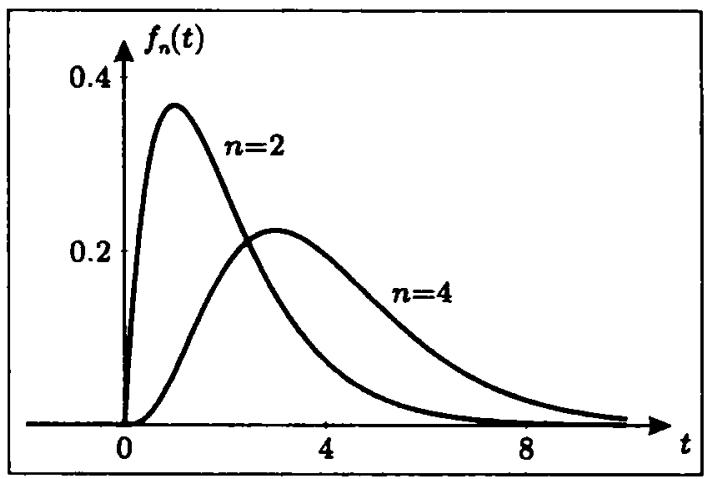
\includegraphics[]{images/chunk1_5255caf9007da5b138c3c00adaa1181c20873509c5b630db8725e3e6d66521b9.jpg}
\end{figure}

\noindent\textbf{Hint:} Use the formula for $P\{\xi_n > t\}$ in the proof of \cref{prop:poisson-process-distribution} to find the distribution function of $\xi_n$. Is this function differentiable? What is the derivative?
\end{Exercise}

\begin{Exercise}
\label{ex:poisson-infinity-limit}
Prove that
\[
\lim_{t \to \infty} N(t) = \infty \quad \text{a.s.}
\]

\noindent\textbf{Hint:} What is the limit of $P\{N(k) \geq n\}$ as $k \to \infty$? Can you express $\{\lim_{t \to \infty} N(t) = \infty\}$ in terms of the sets $\{N(k) \geq n\}$?
\end{Exercise}

\begin{Exercise}
\label{ex:poisson-odd-even}
Verify that
\[
P\{N(t) \text{ is odd}\} = e^{-\lambda t} \sinh(\lambda t),
\]
\[
P\{N(t) \text{ is even}\} = e^{-\lambda t} \cosh(\lambda t).
\]

\noindent\textbf{Hint:} What is the probability that $N(t) = 2n + 1$? Compare this to the $n$-th term of the Taylor expansion of $\sinh(\lambda t)$.
\end{Exercise}

\begin{Exercise}
\label{ex:poisson-strong-law}
Show that
\[
\lim_{t \to \infty} \frac{N(t)}{t} = \lambda \quad \text{a.s.}
\]
if $N(t)$ is a Poisson process with parameter $\lambda$.

\noindent\textbf{Hint:} $N(n)$ is the sum of independent identically distributed random variables $N(1), N(2) - N(1), \ldots, N(n) - N(n-1)$, so the strong law of large numbers can be applied to obtain the limit of $N(n)/n$ as $n \to \infty$. Because $N(t)$ is non-decreasing, the limit will not be affected if $n$ is replaced by a continuous parameter $t \geq 0$.
\end{Exercise}

\section{Brownian Motion}
\label{sec:brownian-motion}

Imagine a cloud of smoke in completely still air. In time, the cloud will spread over a large volume, the concentration of smoke varying in a smooth manner. However, if a single smoke particle is observed, its path turns out to be extremely rough due to frequent collisions with other particles. This exemplifies two aspects of the same phenomenon called diffusion: erratic particle trajectories at the microscopic level, giving rise to a very smooth behaviour of the density of the whole ensemble of particles. The Wiener process $W(t)$ defined below is a mathematical device designed as a model of the motion of individual diffusing particles. In particular, its paths exhibit similar erratic behaviour to the trajectories of real smoke particles. Meanwhile, the density $f_{W(t)}$ of the random variable $W(t)$ is very smooth, given by the exponential function
\begin{equation}
f_{W(t)}(x) = \frac{1}{\sqrt{2\pi t}} e^{-\frac{x^2}{2t}},
\label{eq:wiener-density}
\end{equation}
which is a solution of the diffusion equation
\begin{equation}
\frac{\partial f}{\partial t} = \frac{1}{2} \frac{\partial^2 f}{\partial x^2}
\label{eq:diffusion-equation}
\end{equation}
and can be interpreted as the density at time $t$ of a cloud of smoke issuing from a single point source at time 0. The Wiener process $W(t)$ is also associated with the name of the British botanist Robert Brown, who around 1827 observed the random movement of pollen particles in water. We shall study mainly the one-dimensional Wiener process, which can be thought of as the projection of the position of a smoke particle onto one of the axes of a coordinate system.

Apart from describing the motion of diffusing particles, the Wiener process is widely applied in mathematical models involving various noisy systems, for example, the behaviour of asset prices at the stock exchange. If the noise in the system is due to a multitude of independent random changes, then the Central Limit Theorem predicts that the net result will have the normal distribution, a property shared by the increments $W(t) - W(s)$ of the Wiener process. This is one of the main reasons of the widespread use of $W(t)$ in mathematical models.

\subsection{Definition and Basic Properties}
\label{sec:wiener-definition}

\begin{Definition}[Wiener Process / Brownian Motion]
\label{def:wiener-process}
The Wiener process (or Brownian motion) is a stochastic process $W(t)$ with values in $\mathbb{R}$ defined for $t \in [0, \infty)$ such that
\begin{enumerate}
\item $W(0) = 0$ a.s.;
\item the sample paths $t \mapsto W(t)$ are a.s. continuous;
\item for any finite sequence of times $0 < t_1 < \cdots < t_n$ and Borel sets $A_1, \ldots, A_n \subset \mathbb{R}$
\[
P\{W(t_1) \in A_1, \ldots, W(t_n) \in A_n\}
\]
\[
= \int_{A_1} \cdots \int_{A_n} p(t_1, 0, x_1) p(t_2 - t_1, x_1, x_2) \cdots
\]
\[
\cdots p(t_n - t_{n-1}, x_{n-1}, x_n) \, dx_1 \cdots dx_n,
\]
where
\begin{equation}
p(t, x, y) = \frac{1}{\sqrt{2\pi t}} e^{-\frac{(x-y)^2}{2t}} \tag{6.5}
\end{align}
defined for any $x, y \in \mathbb{R}$ and $t > 0$ is called the transition density.
\end{enumerate}
\end{Definition}

A typical sample path of the Wiener process is shown in \cref{fig:wiener-path}.

\begin{figure}[htbp]
\centering
\caption{A typical path of $W(t)$}
\label{fig:wiener-path}
% 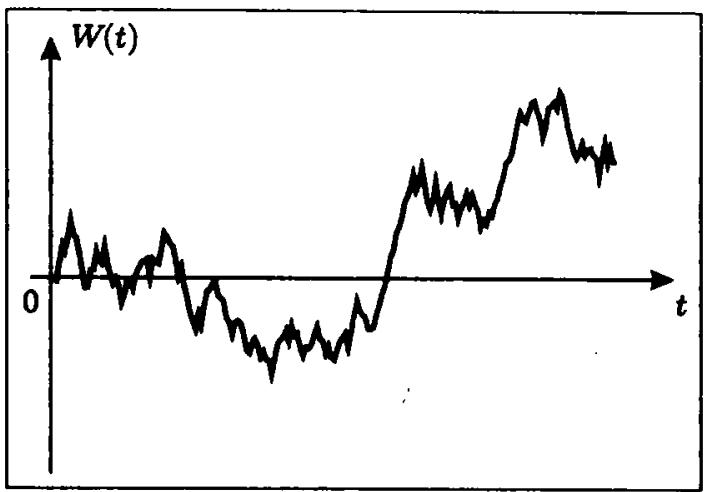
\includegraphics[]{images/chunk1_877c4ec58cf142fcdbc8c04bd3c2b6ce318e0daaa46be271983b945b6c625b81.jpg}
\end{figure}

\begin{Exercise}
\label{ex:wiener-density-expectation-variance}
Show that
\[
f_{W(t)}(x) = \frac{1}{\sqrt{2\pi t}} e^{-\frac{x^2}{2t}}
\]
is the probability density of $W(t)$ and find the expectation and variance of $W(t)$.

\noindent\textbf{Hint:} The density of $W(t)$ can be obtained from condition 3) of \cref{def:wiener-process} written for a single time $t$ and a single Borel set. You will need the formula
\[
\int_{-\infty}^{+\infty} e^{-\frac{x^2}{2}} \, dx = \sqrt{2\pi}
\]
to compute the integrals in the expressions for the expectation and variance.
\end{Exercise}

\begin{remark}
\label{rem:wiener-normal}
The results of Exercise~\ref{ex:wiener-density-expectation-variance} mean that $W(t)$ has the normal distribution with mean 0 and variance $t$.
\end{remark}

\begin{Exercise}
\label{ex:wiener-correlation}
Show that
\[
E(W(s) W(t)) = \min\{s, t\}.
\]

\noindent\textbf{Hint:} The joint density of $W(s)$ and $W(t)$ will be needed. It can be found from condition 3) of \cref{def:wiener-process} written for two times $s$ and $t$ and two Borel sets.
\end{Exercise}

\begin{Exercise}
\label{ex:wiener-increment-mse}
Show that
\[
E\left(|W(t) - W(s)|^2\right) = |t - s|.
\]

\noindent\textbf{Hint:} Expand the square and use the formula in Exercise~\ref{ex:wiener-correlation}.
\end{Exercise}

\begin{Exercise}
\label{ex:wiener-characteristic}
Compute the characteristic function $E(\exp(i\lambda W(t)))$ for any $\lambda \in \mathbb{R}$.

\noindent\textbf{Hint:} Use the density of $W(t)$ found in Exercise~\ref{ex:wiener-density-expectation-variance}.
\end{Exercise}

\begin{Exercise}
\label{ex:wiener-fourth-moment}
Find $E(W(t)^4)$.

\noindent\textbf{Hint:} This can be done, for example, by expressing the expectation in terms of the density of $W(t)$ and computing the resulting integral, or by computing the fourth derivative of the characteristic function of $W(t)$ at 0. The second method is more efficient.
\end{Exercise}

\begin{Definition}[$n$-dimensional Wiener Process]
\label{def:n-dimensional-wiener}
We call $W(t) = (W^1(t), \ldots, W^n(t))$ an $n$-dimensional Wiener process if $W^1(t), \ldots, W^n(t)$ are independent $\mathbb{R}$-valued Wiener processes.
\end{Definition}

\begin{Exercise}
\label{ex:2d-wiener-probability}
For a two-dimensional Wiener process $W(t) = (W^1(t), W^2(t))$ find the probability that $|W(t)| < R$, where $R > 0$ and $|x|$ is the Euclidean norm of $x = (x^1, x^2)$ in $\mathbb{R}^2$, i.e. $|x|^2 = (x^1)^2 + (x^2)^2$.

\noindent\textbf{Hint:} Express the probability in terms of the joint density of $W^1(t)$ and $W^2(t)$. Independence means that the joint density of $W^1(t)$ and $W^2(t)$ is the product of their respective densities, which are known from Exercise~\ref{ex:wiener-density-expectation-variance}. It is convenient to use polar coordinates to compute the resulting integral over a disc.
\end{Exercise}

\subsection{Increments of Brownian Motion}
\label{sec:brownian-increments}

\begin{Proposition}[Increments are Normal]
\label{prop:wiener-increments-normal}
For any $0 \leq s < t$ the increment $W(t) - W(s)$ has the normal distribution with mean 0 and variance $t - s$.
\end{Proposition}

\beginproof
By condition 3) of \cref{def:wiener-process} the joint density of $W(s), W(t)$ is
\[
f_{W(s), W(t)}(x, y) = p(s, 0, x) p(t - s, x, y).
\]

Hence, for any Borel set $A$
\begin{align}
\begin{aligned}
P\{W(t) - W(s) \in A\} &= \int_{\{(x,y): y-x \in A\}} p(s, 0, x) p(t - s, x, y) \, dx \, dy \\
&= \int_{-\infty}^{+\infty} p(s, 0, x) \left(\int_{\{y: y-x \in A\}} p(t - s, x, y) \, dy\right) dx \\
&= \int_{-\infty}^{+\infty} p(s, 0, x) \left(\int_A p(t - s, x, x+u) \, du\right) dx \\
&= \int_{-\infty}^{+\infty} p(s, 0, x) \left(\int_A p(t - s, 0, u) \, du\right) dx \\
&= \int_A p(t - s, 0, u) \, du \int_{-\infty}^{+\infty} p(s, 0, x) \, dx \\
&= \int_A p(t - s, 0, u) \, du.
\end{aligned}
\end{equation}

But $f(u) = p(t - s, 0, u)$ is the density of the normal distribution with mean 0 and variance $t - s$, which proves the claim.
\endproof

\begin{Corollary}
\label{cor:wiener-stationary-increments}
\cref{prop:wiener-increments-normal} implies that $W(t)$ has stationary increments.
\end{Corollary}

\begin{Proposition}[Independent Increments]
\label{prop:wiener-independent-increments}
For any $0 = t_0 \leq t_1 \leq \cdots \leq t_n$ the increments
\[
W(t_1) - W(t_0), \ldots, W(t_n) - W(t_{n-1})
\]
are independent.
\end{Proposition}

\beginproof
From \cref{prop:wiener-increments-normal} we know that the increments of $W(t)$ have the normal distribution. Because normally distributed random variables are independent if and only if they are uncorrelated, it suffices to verify that
\[
E[(W(u) - W(t))(W(s) - W(r))] = 0
\]
for any $0 \leq r \leq s \leq t \leq u$. But this follows immediately from Exercise~\ref{ex:wiener-correlation}:
\begin{equation}
\begin{aligned}
E[(W(u) - W(t))(W(s) - W(r))] &= E(W(u)W(s)) - E(W(u)W(r)) \\
&\quad - E(W(t)W(s)) + E(W(t)W(r)) \\
&= s - r - s + r \\
&= 0,
\end{aligned}
\end{equation}
as required.
\endproof

\begin{Corollary}
\label{cor:wiener-increment-independent-filtration}
For any $0 \leq s < t$ the increment $W(t) - W(s)$ is independent of the $\sigma$-field
\[
\mathcal{F}_s = \sigma\{W(r): 0 \leq r \leq s\}.
\]
\end{Corollary}

\beginproof
By \cref{prop:wiener-independent-increments} the random variables $W(t) - W(s)$ and $W(r) - W(0) = W(r)$ are independent if $0 \leq r \leq s \leq t$. Because the $\sigma$-field $\mathcal{F}_s$ is generated by such $W(r)$, it follows that $W(t) - W(s)$ is independent of $\mathcal{F}_s$.
\endproof

\begin{Exercise}
\label{ex:wiener-martingale}
Show that $W(t)$ is a martingale with respect to the filtration $\mathcal{F}_t$.

\noindent\textbf{Hint:} Take advantage of the fact that $W(t) - W(s)$ is independent of $\mathcal{F}_s$ if $s < t$.
\end{Exercise}

\begin{Exercise}
\label{ex:wiener-squared-martingale}
Show that $|W(t)|^2 - t$ is a martingale with respect to the filtration $\mathcal{F}_t$.

\noindent\textbf{Hint:} Once again, use the fact that $W(t) - W(s)$ is independent of $\mathcal{F}_s$ if $s < t$.
\end{Exercise}

Let us state without proof the following useful characterization of the Wiener process in terms of its increments.

\begin{Theorem}[Wiener Process Characterization]
\label{thm:wiener-characterization}
A stochastic process $W(t), t \geq 0$, is a Wiener process if and only if the following conditions hold:
\begin{enumerate}
\item $W(0) = 0$ a.s.;
\item the sample paths $t \mapsto W(t)$ are continuous a.s.;
\item $W(t)$ has stationary independent increments;
\item the increment $W(t) - W(s)$ has the normal distribution with mean 0 and variance $t - s$ for any $0 \leq s < t$.
\end{enumerate}
\end{Theorem}

\begin{Exercise}
\label{ex:wiener-time-shift}
Show that for any $T > 0$
\[
V(t) = W(t + T) - W(T)
\]
is a Wiener process if $W(t)$ is.

\noindent\textbf{Hint:} Are the increments of $V(t)$ independent? What is their distribution? Does $V(t)$ have continuous paths? Is it true that $V(0) = 0$?
\end{Exercise}

The Wiener process can also be characterized by its martingale properties. The following theorem is also given without proof.

\begin{Theorem}[Lévy's Martingale Characterization]
\label{thm:levy-martingale-characterization}
Let $W(t), t \geq 0$, be a stochastic process and let $\mathcal{F}_t = \sigma(W_s, s \leq t)$ be the filtration generated by it. Then $W(t)$ is a Wiener process if and only if the following conditions hold:
\begin{enumerate}
\item $W(0) = 0$ a.s.;
\item the sample paths $t \mapsto W(t)$ are continuous a.s.;
\item $W(t)$ is a martingale with respect to the filtration $\mathcal{F}_t$;
\item $|W(t)|^2 - t$ is a martingale with respect to $\mathcal{F}_t$.
\end{enumerate}
\end{Theorem}

\begin{Exercise}
\label{ex:wiener-scaling}
Let $c > 0$. Show that $V(t) = \frac{1}{c} W(c^2 t)$ is a Wiener process if $W(t)$ is.

\noindent\textbf{Hint:} Is $V(t)$ a martingale? With respect to which filtration? Is $|V(t)|^2 - t$ a martingale? Are the paths of $V(t)$ continuous? Is it true that $V(0) = 0$?
\end{Exercise}

\subsection{Sample Paths}
\label{sec:brownian-sample-paths}

Let
\[
0 = t_0^n < t_1^n < \dots < t_n^n = T,
\]
where
\[
t_i^n = \frac{iT}{n},
\]
be a partition of the interval $[0, T]$ into $n$ equal parts. We denote by
\[
\Delta_i^n W = W(t_{i+1}^n) - W(t_i^n)
\]
the corresponding increments of the Wiener process $W(t)$.

\begin{Exercise}
\label{ex:wiener-quadratic-variation}
Show that
\[
\lim_{n \to \infty} \sum_{i=0}^{n-1} (\Delta_i^n W)^2 = T \quad \text{in } L^2.
\]

\noindent\textbf{Hint:} You need to show that
\[
\lim_{n \to \infty} E\left(\left[\sum_{i=0}^{n-1} (\Delta_i^n W)^2 - T\right]^2\right) = 0.
\]
Use the independence of increments to simplify the expectation. What are the expectations of $\Delta_i^n W$, $(\Delta_i^n W)^2$ and $(\Delta_i^n W)^4$?
\end{Exercise}

The next theorem on the variation of the paths of $W(t)$ is a consequence of the result in Exercise~\ref{ex:wiener-quadratic-variation}. First, let us recall that the variation of a function is defined as follows.

\begin{Definition}[Variation]
\label{def:variation}
The variation of a function $f: [0,T] \to \mathbb{R}$ is defined to be
\[
\limsup_{\Delta t \to 0} \sum_{i=0}^{n-1} |f(t_{i+1}) - f(t_i)|,
\]
where $t = (t_0, t_1, \ldots, t_n)$ is a partition of $[0, T]$, i.e. $0 = t_0 < t_1 < \cdots < t_n = T$, and where
\[
\Delta t = \max_{i=0, \ldots, n-1} |t_{i+1} - t_i|.
\]
\end{Definition}

\begin{Theorem}[Infinite Variation]
\label{thm:wiener-infinite-variation}
The variation of the paths of $W(t)$ is infinite a.s.
\end{Theorem}

\beginproof
Consider the sequence of partitions $t^n = (t_0^n, t_1^n, \ldots, t_n^n)$ of $[0, T]$ into $n$ equal parts. Then
\[
\sum_{i=0}^{n-1} |\Delta_i^n W|^2 \leq \left(\max_{i=0, \ldots, n-1} |\Delta_i^n W|\right) \sum_{i=0}^{n-1} |\Delta_i^n W|.
\]

Since the paths of $W(t)$ are a.s. continuous on $[0, T]$,
\[
\lim_{n \to \infty} \left(\max_{i=0, \ldots, n-1} |\Delta_i^n W|\right) = 0 \quad \text{a.s.}
\]

By Exercise~\ref{ex:wiener-quadratic-variation} there is a subsequence $t^{n_k} = (t_0^{n_k}, t_1^{n_k}, \ldots, t_{n_k}^{n_k})$ of partitions such that
\[
\lim_{k \to \infty} \sum_{i=0}^{n_k-1} |\Delta_i^{n_k} W|^2 = T \quad \text{a.s.}
\]

This is because every sequence of random variables convergent in $L^2$ has a subsequence convergent a.s. It follows that
\[
\lim_{k \to \infty} \sum_{i=0}^{n_k-1} |\Delta_i^{n_k} W| = \infty \quad \text{a.s.},
\]
while
\[
\lim_{k \to \infty} \Delta t^{n_k} = \lim_{k \to \infty} \frac{T}{n_k} = 0,
\]
which proves the theorem.
\endproof

\cref{thm:wiener-infinite-variation} has important consequences for the theory of stochastic integrals presented in the next chapter. This is because an integral of the form
\[
\int_0^T f(t) \, dW(t)
\]
cannot be defined pathwise (that is, separately for each $\omega \in \Omega$) as the Riemann-Stieltjes integral if the paths have infinite variation. It turns out that an intrinsically stochastic approach will be needed to tackle such integrals, see \cref{chap:stochastic-calculus}.

\begin{Exercise}
\label{ex:wiener-nondifferentiable-zero}
Show that $W(t)$ is a.s. non-differentiable at $t = 0$.

\noindent\textbf{Hint:} By Exercise~\ref{ex:wiener-scaling} $V_c(t) = \frac{1}{c} W(c^2 t)$ is a Wiener process for any $c > 0$. Deduce that the probability
\[
P\left\{\frac{|W(t)|}{t} > cM \text{ for some } t \in [0, \frac{1}{c^2}]\right\}
\]
is the same for each $c > 0$. What is the probability that the limit of $\frac{|W(t)|}{t}$ exists as $t \searrow 0$, then?
\end{Exercise}

\begin{Exercise}
\label{ex:wiener-nondifferentiable-general}
Show that for any $t \geq 0$ the Wiener process $W(t)$ is a.s. non-differentiable at $t$.

\noindent\textbf{Hint:} $V_t(s) = W(s + t) - W(t)$ is a Wiener process for any $t \geq 0$.
\end{Exercise}

A weak point in the assertion in Exercise~\ref{ex:wiener-nondifferentiable-general} is that for each $t$ the event of measure 1 in which $W(t)$ is non-differentiable at $t$ may turn out to be different for each $t \geq 0$. The theorem below, which is presented without proof, shows that in fact the same event of measure 1 can be chosen for each $t \geq 0$. This is not a trivial conclusion because the set of $t \geq 0$ is uncountable.

\begin{Theorem}
\label{thm:wiener-nondifferentiable-everywhere}
With probability 1 the Wiener process $W(t)$ is non-differentiable at any $t \geq 0$.
\end{Theorem}

\subsection{Doob's Maximal $L^2$ Inequality for Brownian Motion}
\label{sec:doob-maximal-inequality}

The inequality proved in this section is necessary to study the properties of stochastic integrals in the next chapter. It can be viewed as an extension of Doob's maximal $L^2$ inequality in \crefythm{thm:doob-maximal-inequality-discrete} to the case of continuous time. In fact, in the result below the Wiener process can be replaced by any square integrable martingale $\xi(t), t \geq 0$ with a.s. continuous paths.

\begin{Theorem}[Doob's Maximal $L^2$ Inequality]
\label{thm:doob-maximal-l2}
For any $t > 0$
\begin{equation}
E\left(\max_{s \leq t} |W(s)|^2\right) \leq 4 E|W(t)|^2. \tag{6.6}
\end{align}
\end{Theorem}

\beginproof
For $t > 0$ and $n \in \mathbb{N}$ we define
\begin{align}
M_k^n = \left|W\left(\frac{kt}{2^n}\right)\right|, \quad 0 \leq k \leq 2^n. \tag{6.7}
\end{align}

Then, by Jensen's inequality, $M_k^n, k = 0, \ldots, 2^n$ is a non-negative square integrable submartingale with respect to the filtration $\mathcal{F}_k^n = \mathcal{F}_{\frac{k+1}{2^n}}$, so by \crefythm{thm:doob-maximal-inequality-discrete}
\[
E\left(\max_{k \leq 2^n} |M_k^n|^2\right) \leq 4 E|M_{2^n}^n|^2 = 4 E|W(t)|^2.
\]

Since $W(t)$ has a.s. continuous paths,
\[
\lim_{n \to \infty} \max_{k \leq 2^n} |M_k^n|^2 = \max_{s \leq t} |W(s)|^2 \quad \text{a.s.}
\]

Moreover, since $M_k^n = M_{2k}^{n+1}$, the sequence $\sup_{k \leq 2^n} |M_k^n|^2, n \in \mathbb{N}$, is increasing. Hence by the Lebesgue monotone convergence theorem $\max_{s \leq t} |W(s)|^2$ is an integrable function and
\[
E\left(\max_{s \leq t} |W(s)|^2\right) = \lim_{n \to \infty} E\left(\max_{k \leq 2^n} |M_k^n|^2\right) \leq 4 E|W(t)|^2,
\]
completing the proof.
\endproof

\subsection{Various Exercises on Brownian Motion}
\label{sec:brownian-exercises}

\begin{Exercise}
\label{ex:diffusion-equation}
Verify that the transition density $p(t, x, y)$ satisfies the diffusion equation
\[
\frac{\partial p}{\partial t} = \frac{1}{2} \frac{\partial^2 p}{\partial y^2}.
\]

\noindent\textbf{Hint:} Simply differentiate the expression \cref{eq:transition-density} for the transition density.
\end{Exercise}

\begin{Exercise}
\label{ex:wiener-negative}
Show that $Z(t) = -W(t)$ is a Wiener process if $W(t)$ is.

\noindent\textbf{Hint:} Are the increments of $Z(t)$ independent? How are they distributed? Are the paths of $Z(t)$ continuous? Is it true that $Z(0) = 0$?
\end{Exercise}

\begin{Exercise}
\label{ex:wiener-conditional-density}
Show that for any $0 \leq s < t$
\[
P\{W(t) \in A \mid W(s)\} = \int_A p(t - s, W(s), y) \, dy.
\]

\noindent\textbf{Hint:} Write the conditional probability as the conditional expectation of $1_A(W(t))$ given $W(s)$. Compute the conditional expectation by transforming the integral of $1_A(W(t))$ over any event in the $\sigma$-field generated by $W(s)$. This can be done using the joint density of $W(s)$ and $W(t)$. Refer to the chapter on conditional expectation if necessary.
\end{Exercise}

\begin{Exercise}
\label{ex:exponential-martingale}
Show that $e^{W(t)} e^{-\frac{t}{2}}$ is a martingale. (It is called the exponential martingale.)

\noindent\textbf{Hint:} What is the expectation of $e^{W(t) - W(s)}$ for $s < t$? By independence it is equal to the conditional expectation of $e^{W(t) - W(s)}$ given $\mathcal{F}_s$. This will give the martingale condition.
\end{Exercise}

\begin{Exercise}
\label{ex:wiener-conditional-expectation}
Compute $E(W(s) \mid W(t))$ for $0 \leq s < t$.

\noindent\textbf{Hint:} You want to find a Borel function $F$ such that $E(W(s) \mid W(t)) = F(W(t))$, i.e.
\[
\int_{\{W(t) \in A\}} W(s) \, dP = \int_{\{W(t) \in A\}} F(W(t)) \, dP.
\]
Either side of this equality can be transformed using the joint density of $W(t)$ and $W(s)$.
\end{Exercise}

\section{Solutions}
\label{sec:chapter-solutions}

\subsection{Solution to Exercise~\ref{ex:exponential-distribution-function}}
\addcontentsline{toc}{subsection}{Solution 6.1}

Suppose that $\eta$ is a random variable with exponential distribution of rate $\lambda$. The distribution function of $\eta$ is
\begin{align}
F(t) = P\{\eta \leq t\} = 1 - P\{\eta > t\} = \begin{cases}
0 & \text{if } t < 0, \\
1 - e^{-\lambda t} & \text{if } t \geq 0.
\end{cases}
\label{eq:exponential-cdf}
\end{equation}

Therefore $\eta$ has density
\begin{equation}
f(t) = \frac{d}{dt} F(t) = \begin{cases}
0 & \text{if } t < 0, \\
\lambda e^{-\lambda t} & \text{if } t > 0.
\end{cases}
\label{eq:exponential-density}
\end{equation}

The distribution function $F(t)$ and density $f(t)$ are shown in \cref{fig:exponential-distribution}.

\begin{figure}[htbp]
\centering
\caption{The distribution function $F(t)$ and density $f(t)$ of a random variable with exponential distribution of rate $\lambda = 2$}
\label{fig:exponential-distribution}
% 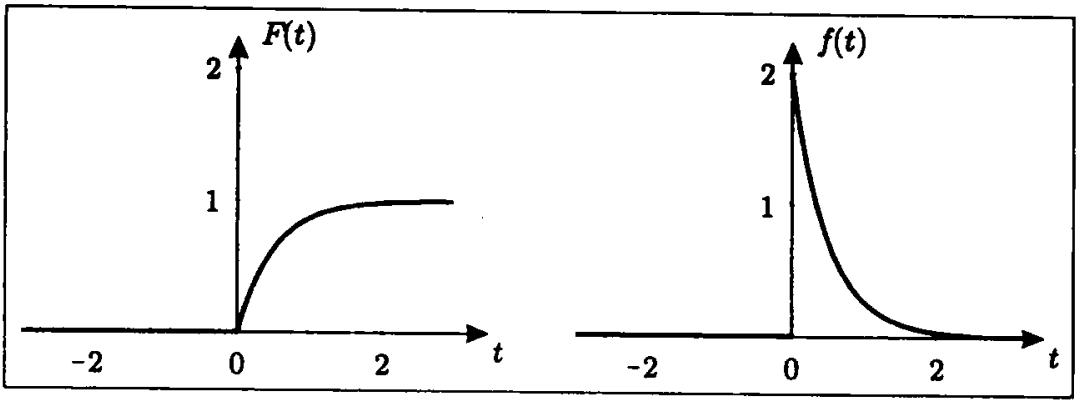
\includegraphics[]{images/chunk1_6f383241ec563e2749359d0d5dfcee8ca02237c4809b65a13fd2f2116b785171.jpg}
\end{figure}

\subsection{Solution to Exercise~\ref{ex:exponential-expectation-variance}}
\addcontentsline{toc}{subsection}{Solution 6.2}

Using the density $f(t) = \lambda e^{-\lambda t}$ found in Exercise~\ref{ex:exponential-distribution-function} and integrating by parts, we obtain
\begin{equation}
\begin{aligned}
E(\eta) &= \int_{-\infty}^{\infty} t f(t) \, dt = \int_0^{\infty} t \lambda e^{-\lambda t} \, dt = -\int_0^{\infty} t \frac{d}{dt} e^{-\lambda t} \, dt \\
&= -t e^{-\lambda t}\Big|_0^{\infty} + \int_0^{\infty} e^{-\lambda t} \, dt = 0 - \frac{1}{\lambda} e^{-\lambda t}\Big|_0^{\infty} = \frac{1}{\lambda}.
\end{aligned}
\label{eq:exponential-expectation}
\end{equation}

In a similar way we compute
\begin{equation}
\begin{aligned}
E(\eta^2) &= \int_{-\infty}^{\infty} t^2 f(t) \, dt = \int_0^{\infty} t^2 \lambda e^{-\lambda t} \, dt = -\int_0^{\infty} t^2 \frac{d}{dt} e^{-\lambda t} \, dt \\
&= -t^2 e^{-\lambda t}\Big|_0^{\infty} + 2\int_0^{\infty} t e^{-\lambda t} \, dt = 0 + \frac{2}{\lambda} \int_0^{\infty} t f(t) \, dt = \frac{2}{\lambda^2}.
\end{aligned}
\label{eq:exponential-second-moment}
\end{equation}

It follows that the variance is equal to
\begin{equation}
\operatorname{var}(\eta) = E(\eta^2) - (E(\eta))^2 = \frac{2}{\lambda^2} - \frac{1}{\lambda^2} = \frac{1}{\lambda^2}.
\label{eq:exponential-variance}
\end{equation}

\subsection{Solution to Exercise~\ref{ex:exponential-functional-equation}}
\addcontentsline{toc}{subsection}{Solution 6.3}

By the definition of a random variable with exponential distribution
\[
P\{\eta > s + t\} = e^{-\lambda(s+t)} = e^{-\lambda s} e^{-\lambda t} = P\{\eta > s\} P\{\eta > t\}.
\]

\subsection{Solution to Exercise~\ref{ex:lack-of-memory-equivalent}}
\addcontentsline{toc}{subsection}{Solution 6.4}

By the definition of conditional probability
\begin{equation}
\begin{aligned}
P\{\eta > t + s \mid \eta > s\} &= \frac{P\{\eta > t + s, \eta > s\}}{P\{\eta > s\}} \\
&= \frac{P\{\eta > t + s\}}{P\{\eta > s\}},
\end{aligned}
\end{equation}
since $\{\eta > t + s, \eta > s\} = \{\eta > t + s\}$ (because $\eta > s + t$ implies that $\eta > s$). Now it is clear that \cref{eq:exponential-functional-equation} is equivalent to \cref{eq:lack-of-memory}.

\subsection{Solution to Exercise~\ref{ex:exponential-unique-lack-of-memory}}
\addcontentsline{toc}{subsection}{Solution 6.5}

The exponential distribution is the only probability distribution satisfying the lack of memory property because the only non-negative non-increasing solutions of the functional equation
\[
g(t + s) = g(t) g(s)
\]
are of the form $g(t) = a^t$ for some $0 \leq a \leq 1$.

To verify this observe that $[g(m/n)]^n = g(m) = [g(1)]^m$ for any integers $m$ and $n \neq 0$. Let $a := g(1)$. It follows that
\[
g(q) = a^q \quad \text{for any } q \in \mathbb{Q}.
\]

Since $g$ is non-increasing, $0 \leq a \leq 1$ and
\[
a^t = \inf_{t > q \in \mathbb{Q}} g(q) \geq g(t) \geq \sup_{t < q \in \mathbb{Q}} g(q) = a^t,
\]
so indeed
\[
g(t) = a^t \quad \text{for any } t \in \mathbb{R}.
\]

As a result, $P\{\eta > t\} = a^t$ for some $0 \leq a \leq 1$. But the distribution function of a random variable cannot be constant, so $0 \neq a \neq 1$. Hence $a = e^{-\lambda}$ for some $\lambda > 0$, completing the argument.

\subsection{Solution to Exercise~\ref{ex:poisson-expectation}}
\addcontentsline{toc}{subsection}{Solution 6.6}

Since $N(t)$ has the Poisson distribution with parameter $\lambda t$ we have $E(N(t)) = \lambda t$. Indeed
\begin{equation}
\begin{aligned}
E(N(t)) &= \sum_{n=0}^{\infty} n P\{N(t) = n\} = \sum_{n=0}^{\infty} n e^{-\lambda t} \frac{(\lambda t)^n}{n!} \\
&= \lambda t e^{-\lambda t} \sum_{n=1}^{\infty} \frac{(\lambda t)^{n-1}}{(n-1)!} = \lambda t e^{-\lambda t} e^{\lambda t} = \lambda t.
\end{aligned}
\end{equation}

\subsection{Solution to Exercise~\ref{ex:poisson-joint-probability}}
\addcontentsline{toc}{subsection}{Solution 6.7}

Using the fact that $\eta_1, \eta_2, \ldots$ are independent and exponentially distributed, we obtain
\begin{equation}
\begin{aligned}
P\{N(s) = 1, N(t) = 2\} &= P\{\xi_1 \leq s < \xi_2 \leq t < \xi_3\} \\
&= P\{\eta_1 \leq s < \eta_1 + \eta_2 \leq t < \eta_1 + \eta_2 + \eta_3\} \\
&= \int_0^s P\{s < u + \eta_2 \leq t < u + \eta_2 + \eta_3\} \lambda e^{-\lambda u} \, du \\
&= \int_0^s \left(\int_{s-u}^{t-u} P\{t < u + v + \eta_3\} \lambda e^{-\lambda v} \, dv\right) \lambda e^{-\lambda u} \, du \\
&= \int_0^s \left(\int_{s-u}^{t-u} e^{-\lambda(t-u-v)} \lambda e^{-\lambda v} \, dv\right) \lambda e^{-\lambda u} \, du \\
&= \lambda^2 e^{-\lambda t} s (t - s).
\end{aligned}
\end{equation}

\subsection{Solution to Exercise~\ref{ex:n-t-equals-difference}}
\addcontentsline{toc}{subsection}{Solution 6.8}

Since
\begin{equation}
\begin{aligned}
\xi_n^t &= \eta_1^t + \dots + \eta_n^t \\
&= \xi_{N(t)+1} - t + \eta_{N(t)+2} + \dots + \eta_{N(t)+n} \\
&= \xi_{N(t)+n} - t,
\end{aligned}
\end{equation}
it follows that
\begin{equation}
\begin{aligned}
N^t(s) &= \max\{n: \xi_n^t \leq s\} \\
&= \max\{n: \xi_{N(t)+n} \leq t + s\} \\
&= \max\{n: \xi_n \leq t + s\} - N(t) \\
&= N(t + s) - N(t).
\end{aligned}
\end{equation}

\subsection{Solution to Exercise~\ref{ex:eta-t-tail-conditional}}
\addcontentsline{toc}{subsection}{Solution 6.9}

It is easily verified that
\[
\{N(t) = n\} = \{\eta_{n+1} > t - \xi_n, t \geq \xi_n\}
\]
\[
\{\eta_1^t > s, N(t) = n\} = \{\eta_{n+1} > s + t - \xi_n, t \geq \xi_n\}
\]

Since $\xi_n, \eta_{n+1}$ are independent and $\eta_{n+1}$ satisfies the lack of memory property from Exercise~\ref{ex:exponential-functional-equation},
\begin{equation}
\begin{aligned}
P\{\eta_1^t > s, N(t) = n\} &= P\{\eta_{n+1} > s + t - \xi_n, t \geq \xi_n\} \\
&= \int_{-\infty}^t P\{\eta_{n+1} > s + t - u\} P_{\xi_n}(du) \\
&= P\{\eta_{n+1} > s\} \int_{-\infty}^t P\{\eta_{n+1} > t - u\} P_{\xi_n}(du) \\
&= P\{\eta_{n+1} > s\} P\{\eta_{n+1} > t - \xi_n, t \geq \xi_n\} \\
&= P\{\eta_{n+1} > s\} P\{N(t) = n\} \\
&= P\{\eta_1 > s\} P\{N(t) = n\}.
\end{aligned}
\end{equation}

The last equality holds because $\eta_{n+1}$ has the same distribution as $\eta_1$. Now divide both sides by $P\{N(t) = n\}$ to get
\[
P\{\eta_1^t > s \mid N(t) = n\} = P\{\eta_1 > s\}
\]
for any $n = 0, 1, 2, \ldots$. As a result,
\[
P\{\eta_1^t > s \mid N(t)\} = P\{\eta_1 > s\}
\]
because $N(t)$ is a discrete random variable with values $0, 1, 2, \ldots$.

\subsection{Solution to Exercise~\ref{ex:eta-t-independence}}
\addcontentsline{toc}{subsection}{Solution 6.10}

As in Solution~\ref{ex:eta-t-tail-conditional},
\[
\{N(t) = n\} = \{\eta_{n+1} > t - \xi_n, t \geq \xi_n\},
\]
\[
\{\eta_1^t > s_1, N(t) = n\} = \{\eta_{n+1} > s_1 + t - \xi_n, t \geq \xi_n\},
\]
and, more generally,
\begin{equation}
\begin{aligned}
&\{\eta_1^t > s_1, \eta_2^t > s_2, \ldots, \eta_k^t > s_k, N(t) = n\} \\
&= \{\eta_{n+1} > s_1 + t - \xi_n, t \geq \xi_n\} \cap \{\eta_{n+2} > s_2\} \cap \cdots \cap \{\eta_{n+k} > s_k\}.
\end{aligned}
\end{equation}

Since $\xi_n, \eta_{n+1}, \ldots, \eta_{n+k}$ are independent and $\eta_{n+2}, \ldots, \eta_{n+k}$ have the same distribution as $\eta_2, \ldots, \eta_k$, using Exercise~\ref{ex:eta-t-tail-conditional} we find that
\begin{equation}
\begin{aligned}
&P\{\eta_1^t > s_1, \eta_2^t > s_2, \ldots, \eta_k^t > s_k, N(t) = n\} \\
&= P\{\eta_{n+1} > s_1 + t - \xi_n, \xi_n \leq t\} P\{\eta_{n+2} > s_2\} \cdots P\{\eta_{n+k} > s_k\} \\
&= P\{\eta_1^t > s_1, N(t) = n\} P\{\eta_2 > s_2\} \cdots P\{\eta_k > s_k\} \\
&= P\{\eta_1^t > s_1 \mid N(t) = n\} P\{\eta_2 > s_2\} \cdots P\{\eta_k > s_k\} P\{N(t) = n\} \\
&= P\{\eta_1 > s_1\} P\{\eta_2 > s_2\} \cdots P\{\eta_k > s_k\} P\{N(t) = n\}.
\end{aligned}
\end{equation}

As in Solution~\ref{ex:eta-t-tail-conditional}, this implies the desired equality.

\subsection{Solution to Exercise~\ref{ex:eta-t-distribution}}
\addcontentsline{toc}{subsection}{Solution 6.11}

Take the expectation on both sides of the equality in Exercise~\ref{ex:eta-t-independence} to find that
\begin{equation}
P\{\eta_1^t > s_1, \ldots, \eta_k^t > s_k\} = P\{\eta_1 > s_1\} \cdots P\{\eta_k > s_k\}.
\end{equation}

If all the numbers $s_n$ except perhaps one are zero, it follows that
\[
P\{\eta_n^t > s_n\} = P\{\eta_n > s_n\}, \quad n = 1, \ldots, k,
\]
so the random variables $\eta_n^t$ have the same distribution as $\eta_n$. Inserting this back into the first equality, we obtain
\[
P\{\eta_1^t > s_1, \ldots, \eta_k^t > s_k\} = P\{\eta_1^t > s_1\} \cdots P\{\eta_k^t > s_k\},
\]
so the $\eta_n^t$ are independent.

To prove that the $\eta_n^t$ are independent of $N(t)$ integrate the formula in Exercise~\ref{ex:eta-t-independence} over $\{N(t) = n\}$ and multiply by $P\{N(t) = n\}$ to get
\[
P\{\eta_1^t > s_1, \ldots, \eta_k^t > s_k, N(t) = n\} = P\{\eta_1 > s_1\} \cdots P\{\eta_k > s_k\} P\{N(t) = n\}.
\]

But $P\{\eta_n^t > s_n\} = P\{\eta_n > s_n\}$, hence $N(t)$ and the $\eta_n^t$ are independent.

\subsection{Solution to Exercise~\ref{ex:poisson-martingale}}
\addcontentsline{toc}{subsection}{Solution 6.12}

We need to verify conditions 1), 2), 3) of \cref{def:martingale}. Clearly, $N(t) - \lambda t$ is $\mathcal{F}_t$-measurable. By Exercise~\ref{ex:poisson-expectation}
\[
E(|N(t)|) = E(N(t)) = \lambda t < \infty,
\]
which means that $N(t)$ is integrable, and so is $N(t) - \lambda t$.

\cref{thm:poisson-independent-increments} implies that $N(t) - N(s)$ is independent of $\mathcal{F}_s$ for any $0 \leq s \leq t$, so
\[
E(N(t) - N(s) \mid \mathcal{F}_s) = E(N(t) - N(s)) = E(N(t)) - E(N(s)) = \lambda t - \lambda s.
\]

It follows that
\[
E(N(t) - \lambda t \mid \mathcal{F}_s) = E(N(s) - \lambda s \mid \mathcal{F}_s) = N(s) - \lambda s,
\]
completing the proof.

\subsection{Solution to Exercise~\ref{ex:jump-times-increasing}}
\addcontentsline{toc}{subsection}{Solution 6.13}

Since $\eta_n = \xi_n - \xi_{n-1}$ and $P\{\eta_n > 0\} = e^0 = 1$,
\[
P\{\xi_0 < \xi_1 < \xi_2 < \cdots\} = P\left(\bigcap_{n=1}^{\infty} \{\eta_n > 0\}\right) = 1.
\]

Here we have used the property that if $P(A_n) = 1$ for all $n = 1, 2, \ldots$, then $P\left(\bigcap_{n=1}^{\infty} A_n\right) = 1$.

\subsection{Solution to Exercise~\ref{ex:jump-times-converge-infinity}}
\addcontentsline{toc}{subsection}{Solution 6.14}

Since
\[
\lim_{n \to \infty} \xi_n = \sum_{n=1}^{\infty} \eta_n,
\]
it follows that
\begin{equation}
\begin{aligned}
\left\{\lim_{n \to \infty} \xi_n < \infty\right\} &\subset \left\{\eta_1, \eta_2, \ldots \text{ is a bounded sequence}\right\} \\
&= \bigcup_{m=1}^{\infty} \bigcap_{n=1}^{\infty} \{\eta_n \leq m\}.
\end{aligned}
\end{equation}

Let us compute the probability of this event. Because $\bigcap_{n=1}^{N} \{\eta_n \leq m\}, N = 1, 2, \ldots$ is a contracting sequence of events,
\begin{equation}
\begin{aligned}
P\left(\bigcap_{n=1}^{\infty} \{\eta_n \leq m\}\right) &= \lim_{N \to \infty} P\left(\bigcap_{n=1}^{N} \{\eta_n \leq m\}\right) \\
&= \lim_{N \to \infty} \prod_{n=1}^{N} P\{\eta_n \leq m\} \\
&= \lim_{N \to \infty} (1 - e^{-\lambda m})^N \\
&= 0.
\end{aligned}
\end{equation}

It follows that
\begin{equation}
\begin{aligned}
P\left(\lim_{n \to \infty} \xi_n < \infty\right) &\leq P\left(\bigcup_{m=1}^{\infty} \bigcap_{n=1}^{\infty} \{\eta_n \leq m\}\right) \\
&\leq \sum_{m=1}^{\infty} P\left(\bigcap_{n=1}^{\infty} \{\eta_n \leq m\}\right) \\
&= 0,
\end{aligned}
\end{equation}
completing the proof.

While it is instructive to work through the above estimates, there exists a much more elegant argument. By the strong law of large numbers
\[
\lim_{n \to \infty} \frac{\xi_n}{n} = \frac{1}{\lambda} \quad \text{a.s.}
\]

Here $\frac{1}{\lambda}$ is the expectation of each of the independent identically distributed random variables $\eta_n$ (see Exercise~\ref{ex:exponential-expectation-variance}). It follows that
\[
\lim_{n \to \infty} \xi_n = \infty \quad \text{a.s.},
\]
as required.

\subsection{Solution to Exercise~\ref{ex:gamma-distribution}}
\addcontentsline{toc}{subsection}{Solution 6.15}

In the proof of \cref{prop:poisson-process-distribution} it was shown that
\[
P\{\xi_n > t\} = e^{-\lambda t} \sum_{k=0}^{n-1} \frac{(\lambda t)^k}{k!}
\]
for $t \geq 0$, see \cref{eq:xi-n-tail-probability}. Therefore the distribution function
\[
F_n(t) = P\{\xi_n \leq t\} = 1 - P\{\xi_n > t\} = e^{-\lambda t} \sum_{k=n}^{\infty} \frac{(\lambda t)^k}{k!}
\]
of $\xi_n$ is differentiable, the density $f_n$ of $\xi_n$ being
\begin{equation}
\begin{aligned}
f_n(t) &= \frac{d}{dt} F_n(t) \\
&= -\lambda e^{-\lambda t} \sum_{k=n}^{\infty} \frac{(\lambda t)^k}{k!} + \lambda e^{-\lambda t} \sum_{k=n}^{\infty} \frac{(\lambda t)^{k-1}}{(k-1)!} \\
&= \lambda e^{-\lambda t} \frac{(\lambda t)^{n-1}}{(n-1)!}
\end{aligned}
\end{equation}
for $t > 0$, and clearly $f_n(t) = 0$ for $t \leq 0$.

\subsection{Solution to Exercise~\ref{ex:poisson-infinity-limit}}
\addcontentsline{toc}{subsection}{Solution 6.16}

Because $N(t)$ has non-decreasing trajectories
\[
\left\{\lim_{t \to \infty} N(t) = \infty\right\} = \bigcap_{n=1}^{\infty} \bigcup_{k=1}^{\infty} \{N(k) \geq n\}.
\]

Also, $\{N(k) \geq n\}, k = 1, 2, \ldots$ is an expanding sequence of events and
\begin{equation}
\begin{aligned}
P\{N(k) \geq n\} &= e^{-\lambda k} \sum_{i=n}^{\infty} \frac{(\lambda k)^i}{i!} \\
&= 1 - e^{-\lambda k} \sum_{i=0}^{n-1} \frac{(\lambda k)^i}{i!} \to 1 \quad \text{as } k \to \infty.
\end{aligned}
\end{equation}

It follows that
\[
P\left\{\bigcup_{k=1}^{\infty} \{N(k) \geq n\}\right\} = 1,
\]
so
\[
P\left\{\lim_{t \to \infty} N(t) = \infty\right\} = P\left\{\bigcap_{n=1}^{\infty} \bigcup_{k=1}^{\infty} \{N(k) \geq n\}\right\} = 1.
\]

\subsection{Solution to Exercise~\ref{ex:poisson-odd-even}}
\addcontentsline{toc}{subsection}{Solution 6.17}

Since
\[
\sinh(x) = \frac{e^x - e^{-x}}{2} = \sum_{n=0}^{\infty} \frac{x^{2n+1}}{(2n+1)!},
\]
\[
\cosh(x) = \frac{e^x + e^{-x}}{2} = \sum_{n=0}^{\infty} \frac{x^{2n}}{(2n)!},
\]
we have
\begin{equation}
\begin{aligned}
P\{N(t) \text{ is odd}\} &= \sum_{n=0}^{\infty} P\{N(t) = 2n+1\} \\
&= \sum_{n=0}^{\infty} e^{-\lambda t} \frac{(\lambda t)^{2n+1}}{(2n+1)!} \\
&= e^{-\lambda t} \sinh(\lambda t),
\end{aligned}
\end{equation}
\begin{equation}
\begin{aligned}
P\{N(t) \text{ is even}\} &= \sum_{n=0}^{\infty} P\{N(t) = 2n\} \\
&= \sum_{n=0}^{\infty} e^{-\lambda t} \frac{(\lambda t)^{2n}}{(2n)!} \\
&= e^{-\lambda t} \cosh(\lambda t).
\end{aligned}
\end{equation}

\subsection{Solution to Exercise~\ref{ex:poisson-strong-law}}
\addcontentsline{toc}{subsection}{Solution 6.18}

We can write
\[
N(n) = N(1) + (N(2) - N(1)) + \cdots + (N(n) - N(n-1)),
\]
where $N(1), N(2) - N(1), N(3) - N(2), \ldots$ is a sequence of independent identically distributed random variables with expectation
\[
E(N(1)) = E(N(2) - N(1)) = E(N(3) - N(2)) = \cdots = \lambda.
\]

By the strong law of large numbers
\begin{equation}
\lim_{n \to \infty} \frac{N(n)}{n} = \lambda \quad \text{a.s.} \tag{6.8}
\end{align}

Now, if $n \leq t \leq n+1$, then $N(n) \leq N(t) \leq N(n+1)$ and
\[
\frac{N(n)}{n+1} \leq \frac{N(t)}{t} \leq \frac{N(n+1)}{n}.
\]

By \cref{eq:slln-poisson} both sides tend to $\lambda$ as $n \to \infty$, implying that
\[
\lim_{t \to \infty} \frac{N(t)}{t} = \lambda \quad \text{a.s.}
\]

\subsection{Solution to Exercise~\ref{ex:wiener-density-expectation-variance}}
\addcontentsline{toc}{subsection}{Solution 6.19}

Condition 3) of \cref{def:wiener-process} implies that
\[
f_{W(t)}(x) = p(t, 0, x)
\]
is the density of $W(t)$. Therefore, integrating by parts, we can compute the expectation
\begin{equation}
\begin{aligned}
E(W(t)) &= \int_{-\infty}^{+\infty} x p(t, 0, x) \, dx \\
&= \frac{1}{\sqrt{2\pi t}} \int_{-\infty}^{+\infty} x e^{-\frac{x^2}{2t}} \, dx \\
&= -\frac{t}{\sqrt{2\pi t}} \int_{-\infty}^{+\infty} \frac{d}{dx} e^{-\frac{x^2}{2t}} \, dx \\
&= -\frac{t}{\sqrt{2\pi t}} e^{-\frac{x^2}{2t}}\Big|_{-\infty}^{+\infty} = 0,
\end{aligned}
\end{equation}
and variance
\begin{equation}
\begin{aligned}
E\left((W(t))^2\right) &= \int_{-\infty}^{+\infty} x^2 p(t, 0, x) \, dx \\
&= \frac{1}{\sqrt{2\pi t}} \int_{-\infty}^{+\infty} x^2 e^{-\frac{x^2}{2t}} \, dx \\
&= -\frac{t}{\sqrt{2\pi t}} \int_{-\infty}^{+\infty} x \frac{d}{dx} e^{-\frac{x^2}{2t}} \, dx \\
&= -\frac{t}{\sqrt{2\pi t}} x e^{-\frac{x^2}{2t}}\Big|_{-\infty}^{+\infty} + \frac{t}{\sqrt{2\pi t}} \int_{-\infty}^{+\infty} e^{-\frac{x^2}{2t}} \, dx \\
&= 0 + \frac{t}{\sqrt{2\pi}} \int_{-\infty}^{+\infty} e^{-\frac{u^2}{2}} \, du = t.
\end{aligned}
\end{equation}

We have used the substitution $u = \frac{x}{\sqrt{t}}$ and the formula stated in the hint.

\subsection{Solution to Exercise~\ref{ex:wiener-correlation}}
\addcontentsline{toc}{subsection}{Solution 6.20}

Suppose that $s < t$. Condition 3) of \cref{def:wiener-process} implies that the joint density of $W(s)$ and $W(t)$ is
\[
f_{W(s), W(t)}(x, y) = p(s, 0, x) p(t - s, x, y).
\]

It follows that
\begin{equation}
\begin{aligned}
E(W(s)W(t)) &= \int_{-\infty}^{+\infty} \int_{-\infty}^{+\infty} x y p(s, 0, x) p(t - s, x, y) \, dx \, dy \\
&= \int_{-\infty}^{+\infty} x p(s, 0, x) \left(\int_{-\infty}^{+\infty} y p(t - s, x, y) \, dy\right) dx \\
&= \int_{-\infty}^{+\infty} x^2 p(s, 0, x) \, dx = s.
\end{aligned}
\end{equation}

This is because by the results of Exercise~\ref{ex:wiener-density-expectation-variance}
\begin{equation}
\begin{aligned}
\int_{-\infty}^{+\infty} y p(t - s, x, y) \, dy &= \int_{-\infty}^{+\infty} (x + u) p(t - s, x, x + u) \, du \\
&= \int_{-\infty}^{+\infty} (x + u) p(t - s, 0, u) \, du \\
&= x \int_{-\infty}^{+\infty} p(t - s, 0, u) \, du + \int_{-\infty}^{+\infty} u p(t - s, 0, u) \, du \\
&= x + 0 = x,
\end{aligned}
\end{equation}
and
\[
\int_{-\infty}^{+\infty} x^2 p(s, 0, x) \, dx = s.
\]

It follows that for arbitrary $s, t \geq 0$
\[
E(W(s)W(t)) = \min\{s, t\}.
\]

\subsection{Solution to Exercise~\ref{ex:wiener-increment-mse}}
\addcontentsline{toc}{subsection}{Solution 6.21}

Suppose that $s \leq t$. Then by Exercise~\ref{ex:wiener-correlation}
\begin{equation}
\begin{aligned}
E\left(|W(t) - W(s)|^2\right) &= E(W(t)^2) - 2E(W(s)W(t)) + E(W(s)^2) \\
&= t - 2s + s = t - s.
\end{aligned}
\end{equation}

In general, for arbitrary $s, t \geq 0$
\[
E\left(|W(t) - W(s)|^2\right) = |t - s|.
\]

\subsection{Solution to Exercise~\ref{ex:wiener-characteristic}}
\addcontentsline{toc}{subsection}{Solution 6.22}

Using the density $f_{W(t)}(x) = p(t,0,x)$ of $W(t)$, we compute
\begin{equation}
\begin{aligned}
E(\exp(i\lambda W(t))) &= \int_{-\infty}^{+\infty} e^{i\lambda x} p(t, 0, x) \, dx \\
&= \frac{1}{\sqrt{2\pi t}} \int_{-\infty}^{+\infty} e^{i\lambda x} e^{-\frac{x^2}{2t}} \, dx \\
&= \frac{1}{\sqrt{2\pi t}} e^{-\frac{\lambda^2 t}{2}} \int_{-\infty}^{+\infty} e^{-\frac{(x - i\lambda t)^2}{2t}} \, dx \\
&= e^{-\frac{\lambda^2 t}{2}}.
\end{aligned}
\end{equation}

\subsection{Solution to Exercise~\ref{ex:wiener-fourth-moment}}
\addcontentsline{toc}{subsection}{Solution 6.23}

Using the formula for the characteristic function of $W(t)$ found in Exercise~\ref{ex:wiener-characteristic}, we compute
\begin{equation}
\begin{aligned}
E(W(t)^4) &= \left.\frac{d^4}{d\lambda^4}\right|_{\lambda=0} E(\exp(i\lambda W(t))) \\
&= \left.\frac{d^4}{d\lambda^4}\right|_{\lambda=0} e^{-\frac{1}{2}\lambda^2 t} \\
&= 3t^2.
\end{aligned}
\end{equation}

\subsection{Solution to Exercise~\ref{ex:2d-wiener-probability}}
\addcontentsline{toc}{subsection}{Solution 6.24}

Since $W^1(t), W^2(t)$ are independent, their joint density is the product of the densities of $W^1(t)$ and $W^2(t)$. Therefore
\begin{equation}
\begin{aligned}
P\{|W(t)| < R\} &= \int_{\{|x| < R\}} p(t, 0, x) p(t, 0, y) \, dx \, dy \\
&= \frac{1}{2\pi t} \int_{\{|x| < R\}} e^{-\frac{x^2+y^2}{2t}} \, dx \, dy \\
&= \frac{1}{2\pi t} \int_0^R \int_0^{2\pi} r e^{-\frac{r^2}{2t}} \, d\varphi \, dr \\
&= -\int_0^R \frac{d}{dr} e^{-\frac{r^2}{2t}} \, dr \\
&= 1 - e^{-\frac{R^2}{2t}}.
\end{aligned}
\end{equation}

We have used the polar coordinates $r, \varphi$ to compute the integral.

\subsection{Solution to Exercise~\ref{ex:wiener-martingale}}
\addcontentsline{toc}{subsection}{Solution 6.25}

For any $0 \leq s < t$
\begin{equation}
\begin{aligned}
E(W(t) \mid \mathcal{F}_s) &= E(W(t) - W(s) \mid \mathcal{F}_s) + E(W(s) \mid \mathcal{F}_s) \\
&= E(W(t) - W(s)) + W(s) \\
&= W(s),
\end{aligned}
\end{equation}
since $W(t) - W(s)$ is independent of $\mathcal{F}_s$ by \cref{cor:wiener-increment-independent-filtration}, $W(s)$ is $\mathcal{F}_s$-measurable and $E(W(t)) = E(W(s)) = 0$.

\subsection{Solution to Exercise~\ref{ex:wiener-squared-martingale}}
\addcontentsline{toc}{subsection}{Solution 6.26}

For any $0 \leq s < t$
\begin{equation}
\begin{aligned}
E(W(t)^2 \mid \mathcal{F}_s) &= E(|W(t) - W(s)|^2 \mid \mathcal{F}_s) + E(2W(t)W(s) \mid \mathcal{F}_s) \\
&\quad - E(W(s)^2 \mid \mathcal{F}_s) \\
&= E(|W(t) - W(s)|^2) + 2W(s)E(W(t) \mid \mathcal{F}_s) - W(s)^2 \\
&= t - s + 2W(s)^2 - W(s)^2 \\
&= t - s + W(s)^2,
\end{aligned}
\end{equation}
since $W(t) - W(s)$ is independent of $\mathcal{F}_s$ and has the normal distribution with mean 0 and variance $t - s$, $W(s)$ is $\mathcal{F}_s$-measurable, and $W(t)$ is a martingale. It follows that
\[
E(W(t)^2 - t \mid \mathcal{F}_s) = W(s)^2 - s,
\]
as required.

\subsection{Solution to Exercise~\ref{ex:wiener-time-shift}}
\addcontentsline{toc}{subsection}{Solution 6.27}

For any $0 \leq t_0 < t_1 < \cdots < t_n$ the increments
\[
V(t_n) - V(t_{n-1}), \ldots, V(t_1) - V(t_0)
\]
of $V(t)$ are independent, since the increments
\[
W(t_n + T) - W(t_{n-1} + T), \ldots, W(t_1 + T) - W(t_0 + T)
\]
of $W(t)$ are independent. For any $0 \leq s < t$ the increment $V(t) - V(s)$ has the normal distribution with mean zero and variance $t - s$, since $W(t + T) - W(s + T)$ does. Moreover, the paths $t \mapsto V(t) = W(t + T) - W(T)$ are continuous and
\[
V(0) = W(T) - W(T) = 0.
\]

By \cref{thm:wiener-characterization} $V(t)$ is a Wiener process.

\subsection{Solution to Exercise~\ref{ex:wiener-scaling}}
\addcontentsline{toc}{subsection}{Solution 6.28}

It is clear that $V(0) = \frac{1}{c} W(0) = 0$ a.s. and the paths $t \mapsto V(t) = \frac{1}{c} W(c^2 t)$ are a.s. continuous. We shall verify that $V(t)$ and $|V(t)|^2 - t$ are martingales with respect to the filtration
\begin{equation}
\begin{aligned}
\mathcal{G}_t &= \sigma\{V(s): 0 \leq s \leq t\} \\
&= \sigma\{W(c^2 s): 0 \leq s \leq t\} \\
&= \sigma\{W(s): 0 \leq s \leq c^2 t\} \\
&= \mathcal{F}_{c^2 t}.
\end{aligned}
\end{equation}

Indeed, if $s < t$, then $c^2 s < c^2 t$, so
\begin{equation}
\begin{aligned}
E(V(t) \mid \mathcal{G}_s) &= E\left(\frac{1}{c} W(c^2 t) \mid \mathcal{F}_{c^2 s}\right) \\
&= \frac{1}{c} E\left(W(c^2 t) \mid \mathcal{F}_{c^2 s}\right) \\
&= \frac{1}{c} W(c^2 s) = V(s),
\end{aligned}
\end{equation}
and
\begin{equation}
\begin{aligned}
E(|V(t)|^2 - t \mid \mathcal{G}_s) &= E\left(\frac{1}{c^2} |W(c^2 t)|^2 - t \mid \mathcal{F}_{c^2 s}\right) \\
&= \frac{1}{c^2} E(|W(c^2 t)|^2 - c^2 t \mid \mathcal{F}_{c^2 s}) \\
&= \frac{1}{c^2}(|W(c^2 s)|^2 - c^2 s) \\
&= |V(s)|^2 - s,
\end{aligned}
\end{equation}
since $W(t)$ and $|W(t)|^2 - t$ are martingales with respect to the filtration $\mathcal{F}_t$. It follows by Lévy's martingale characterization that $V(t)$ is a Wiener process.

\subsection{Solution to Exercise~\ref{ex:wiener-quadratic-variation}}
\addcontentsline{toc}{subsection}{Solution 6.29}

Since the increments $\Delta_i^n W$ are independent and
\[
E(\Delta_i^n W) = 0, \quad E\left((\Delta_i^n W)^2\right) = \frac{T}{n}, \quad E\left((\Delta_i^n W)^4\right) = \frac{3T^2}{n^2},
\]
it follows that
\begin{equation}
\begin{aligned}
E\left(\left[\sum_{i=0}^{n-1} (\Delta_i^n W)^2 - T\right]^2\right) &= E\left(\left[\sum_{i=0}^{n-1} \left((\Delta_i^n W)^2 - \frac{T}{n}\right)\right]^2\right) \\
&= \sum_{i=0}^{n-1} E\left[\left((\Delta_i^n W)^2 - \frac{T}{n}\right)^2\right] \\
&= \sum_{i=0}^{n-1} \left[E\left((\Delta_i^n W)^4\right) - \frac{2T}{n}E\left((\Delta_i^n W)^2\right) + \frac{T^2}{n^2}\right] \\
&= \sum_{i=0}^{n-1} \left[\frac{3T^2}{n^2} - \frac{2T^2}{n^2} + \frac{T^2}{n^2}\right] = \frac{2T^2}{n} \to 0,
\end{aligned}
\end{equation}
as $n \to \infty$.

\subsection{Solution to Exercise~\ref{ex:wiener-nondifferentiable-zero}}
\addcontentsline{toc}{subsection}{Solution 6.30}

We claim that, with probability 1, for any positive integer $n$ there is a $t \in [0, \frac{1}{n^4}]$ such that $\frac{|W(t)|}{t} > n$. This condition implies that $W(t)$ is not differentiable at $t = 0$.

Let us put
\[
A_n = \left\{\frac{|W(t)|}{t} > n \text{ for some } t \in [0, \frac{1}{n^4}]\right\}.
\]

By Exercise~\ref{ex:wiener-scaling}
\[
V_n(t) = \frac{1}{n^2} W(n^4 t)
\]
is a Brownian motion for any $n$. Therefore
\begin{equation}
\begin{aligned}
P(A_n) &\geq P\left\{\frac{|W(1/n^4)|}{1/n^4} > n\right\} \\
&= P\left\{\frac{|V_n(1/n^4)|}{1/n^4} > n\right\} \\
&= P\{|W(1)| > \frac{1}{n}\} \to 1 \quad \text{as } n \to \infty.
\end{aligned}
\end{equation}

Since $A_1, A_2, \ldots$ is a contracting sequence of events,
\[
P\left(\bigcap_{n=1}^{\infty} A_n\right) = \lim_{n \to \infty} P(A_n) = 1,
\]
which proves the claim.

\subsection{Solution to Exercise~\ref{ex:wiener-nondifferentiable-general}}
\addcontentsline{toc}{subsection}{Solution 6.31}

By Exercise~\ref{ex:wiener-time-shift} $V_t(s) = W(s + t) - W(t)$ is a Wiener process for any $t \geq 0$. Therefore, by Exercise~\ref{ex:wiener-nondifferentiable-zero} $V_t(s)$ is a.s. non-differentiable at $s = 0$. But this implies that $W(t)$ is a.s. non-differentiable at $t$.

\subsection{Solution to Exercise~\ref{ex:diffusion-equation}}
\addcontentsline{toc}{subsection}{Solution 6.32}

Differentiating
\[
p(t, x, y) = \frac{1}{\sqrt{2\pi t}} e^{-\frac{(y-x)^2}{2t}},
\]
we obtain
\[
\frac{\partial}{\partial t} p(t, x, y) = \frac{y^2 - 2yx + x^2 - t}{2t^2} p(t, x, y),
\]
\[
\frac{\partial}{\partial y} p(t, x, y) = \frac{x - y}{t} p(t, x, y),
\]
\[
\frac{\partial^2}{\partial y^2} p(t, x, y) = \frac{y^2 - 2yx + x^2 - t}{t^2} p(t, x, y),
\]
so
\[
\frac{\partial p}{\partial t} = \frac{1}{2} \frac{\partial^2 p}{\partial y^2},
\]
as required.

\subsection{Solution to Exercise~\ref{ex:wiener-negative}}
\addcontentsline{toc}{subsection}{Solution 6.33}

Clearly, $Z(t) = -W(t)$ has a.s. continuous trajectories and $Z(0) = -W(0) = 0$ a.s. If $W(t)$ has stationary independent increments, then so does $Z(t) = -W(t)$. Finally,
\[
Z(t) - Z(s) = -(W(t) - W(s))
\]
has the same distribution as $W(t) - W(s)$, i.e. normal with mean 0 and variance $t - s$. By \cref{thm:wiener-characterization} $Z(t)$ is a Wiener process.

\subsection{Solution to Exercise~\ref{ex:wiener-conditional-density}}
\addcontentsline{toc}{subsection}{Solution 6.34}

Let $0 \leq s < t$. Then
\begin{equation}
\begin{aligned}
\int_{\{W(s) \in B\}} 1_A(W(t)) \, dP &= P\{W(s) \in B, W(t) \in A\} \\
&= \int_B \int_A p(s, 0, x) p(t - s, x, y) \, dx \, dy \\
&= \int_B \left(\int_A p(t - s, x, y) \, dy\right) p(s, 0, x) \, dx \\
&= \int_{\{W(s) \in B\}} \left(\int_A p(t - s, W(s), y) \, dy\right) \, dP,
\end{aligned}
\end{equation}
for any Borel set $B \subset \mathbb{R}$. It follows that
\[
P\{W(t) \in A \mid W(s)\} = E(1_A(W(t)) \mid W(s)) = \int_A p(t - s, W(s), y) \, dy.
\]

\subsection{Solution to Exercise~\ref{ex:exponential-martingale}}
\addcontentsline{toc}{subsection}{Solution 6.35}

We shall prove that $e^{W(t)} e^{-\frac{t}{2}}$ is a martingale with respect to the filtration $\mathcal{F}_t$. Clearly, it is adapted to the filtration $\mathcal{F}_t$, since $W(t)$ is. Let $0 \leq s < t$. Because $W(t) - W(s)$ is independent of $\mathcal{F}_s$ and $W(s)$ is $\mathcal{F}_s$-measurable,
\begin{equation}
\begin{aligned}
E\left(e^{W(t)} \mid \mathcal{F}_s\right) &= E\left(e^{W(t) - W(s)} e^{W(s)} \mid \mathcal{F}_s\right) \\
&= e^{W(s)} E\left(e^{W(t) - W(s)} \mid \mathcal{F}_s\right) \\
&= e^{W(s)} E\left(e^{W(t) - W(s)}\right).
\end{aligned}
\end{equation}

The increment $W(t) - W(s)$ has the normal distribution with mean 0 and variance $t - s$, so the expectation of $e^{W(t) - W(s)}$ is equal to
\begin{equation}
\begin{aligned}
E\left(e^{W(t) - W(s)}\right) &= \int_{-\infty}^{+\infty} e^x p(t - s, 0, x) \, dx \\
&= e^{\frac{t-s}{2}} \int_{-\infty}^{+\infty} p(t - s, 0, x - t) \, dx \\
&= e^{\frac{t-s}{2}}.
\end{aligned}
\end{equation}

It follows that
\[
E\left(e^{W(t)} e^{-\frac{t}{2}} \mid \mathcal{F}_s\right) = e^{W(s)} e^{-\frac{s}{2}}.
\]

It also follows that $e^{W(t)} e^{-\frac{t}{2}}$ is integrable. Therefore $e^{W(t)} e^{-\frac{t}{2}}$ is a martingale.

\subsection{Solution to Exercise~\ref{ex:wiener-conditional-expectation}}
\addcontentsline{toc}{subsection}{Solution 6.36}

Let $0 \leq s < t$. We are looking for a Borel function $F$ such that $E(W(s) \mid W(t)) = F(W(t))$, i.e.
\[
\int_{\{W(t) \in A\}} W(s) \, dP = \int_{\{W(t) \in A\}} F(W(t)) \, dP
\]
for any Borel set $A$ in $\mathbb{R}$. The integral on the right-hand side can be written as
\[
\int_{\{W(t) \in A\}} F(W(t)) \, dP = \int_A F(y) p(t, 0, y) \, dy,
\]
and the integral on the left-hand side as
\[
\int_{\{W(t) \in A\}} W(s) \, dP = \int_A \left(\int_{-\infty}^{+\infty} x p(s, 0, x) p(t - s, x, y) \, dx\right) dy,
\]
using the expression for the joint density of $W(s)$ and $W(t)$ in Solution~\ref{ex:wiener-correlation}. Let us compute the inner integral:
\begin{equation}
\begin{aligned}
\int_{-\infty}^{+\infty} x p(s, 0, x) p(t - s, x, y) \, dx &= p(t, 0, y) \int_{-\infty}^{+\infty} x p\left(\frac{s(t-s)}{t}, \frac{s}{t} y, x\right) dx \\
&= \frac{s}{t} y p(t, 0, y).
\end{aligned}
\end{equation}

(To see that the first equality holds, just use formula \cref{eq:transition-density} for $p(t, x, y)$.) Therefore
\[
\int_{\{W(t) \in A\}} W(s) \, dP = \int_A \frac{s}{t} y p(t, 0, y) \, dy.
\]

It follows that $F(y) = \frac{s}{t} y$, i.e.
\[
E(W(s) \mid W(t)) = \frac{s}{t} W(t).
\]
